% --------------------------------------------------------------
% This is all preamble stuff that you don't have to worry about.
% Head down to where it says "Start here"
% --------------------------------------------------------------

\documentclass[12pt]{article}

\usepackage[margin=1in]{geometry}
\usepackage{amsmath,amsthm,amssymb}
\usepackage{graphicx}
\usepackage{subcaption}
\usepackage{algorithmicx}
\usepackage{algorithm}
\usepackage{algpseudocode}
\usepackage[colorlinks,linkcolor=blue]{hyperref}
\usepackage[noabbrev]{cleveref}
\usepackage{courier}
\usepackage{listings}


\oddsidemargin 0in
\evensidemargin 0in
\textwidth 6.5in
\topmargin -0.5in
\textheight 9.0in
\graphicspath{./images/}

\newcommand{\ignore}[1]{}
\def\pp{\par\noindent}

\newcommand{\assignment}[4]{
\thispagestyle{plain}
\newpage
\setcounter{page}{1}
\noindent
\begin{center}
\framebox{ \vbox{ \hbox to 6.28in
{CIS 419/519: Applied Machine Learning \hfill #1}
\vspace{4mm}
\hbox to 6.28in
{\hspace{2.5in}\large\bf\mbox{Homework #2}}
\vspace{4mm}
\hbox to 6.28in
{{\it Handed Out: #3 \hfill Due: #4}}
}}
\end{center}
}

\makeatletter
\renewcommand{\fnum@algorithm}{\fname@algorithm}
\makeatother

\lstset{basicstyle=\footnotesize\ttfamily,breaklines=true}
\lstset{framextopmargin=50pt,frame=bottomline}


\begin{document}

\assignment{Fall 2024}{0}{August 28}{7:59 pm September 4}

% --------------------------------------------------------------
%                         Start here
% --------------------------------------------------------------


{\bf Name: }  Yueyang Li    

{\bf PennKey:} ezel22

{\bf PennID:} 47700221

\section{Declaration}
\begin{itemize}
\item \textbf{Person(s) discussed with:} \textit{Your answer}
\item \textbf{Affiliation to the course: student, TA, prof etc.} \textit{Your answer}
\item \textbf{Which question(s) in coding / written HW did you discuss?} \textbf{\textit{Your answer}}
\item \textbf{Briefly explain what was discussed.} \textit{Your answer}
\end{itemize}

\section{Multiple Choice \& Written Questions}

\begin{enumerate}
\item 
\begin{enumerate}
\item C
\item C
\end{enumerate}

\item
\begin{enumerate}
\item D
\item A
\end{enumerate}

\item
  \begin{enumerate}
  \item A
  \item A
  \end{enumerate}

\item
  \begin{enumerate}
  \item B
  \item 
  $Var(X)
  \\= E[(X - E[X])^2] 
  \\= E[X^2 - 2E[X]X + (E[X])^2] 
  \\= E[X^2] - 2E[X]E[X] + (E[X])^2
  \\= E[X^2] - 0 + (E[X])^2
  \\= E[X^2]  + (E[X])^2
  \\ Q.E.D
  $
  \end{enumerate}
 \item
 \begin{enumerate}
     \item C
     \item D
     \item A
 \end{enumerate}

\item 
\begin{enumerate}
\item
    Need to find $\lambda$ such that\\
    $det(A - I\lambda) = 0$
    hence the eigenvalue can be calculated as:\\
    $(4 - \lambda)(5 - \lambda)  - 2 = 0$\\
    $\lambda = 3 \text{ or } \lambda = 6$
    
\item
    Since by the Rayleigh's Quotient, the probable maximum value of this function
    is just the largest Eigenvalue, hence it should just be $6$ but there's no such answers 
    from the list
    

\end{enumerate}

\end{enumerate}


\section{Python Programming Questions}

% Complete questions in your iPython notebook and place all results here.
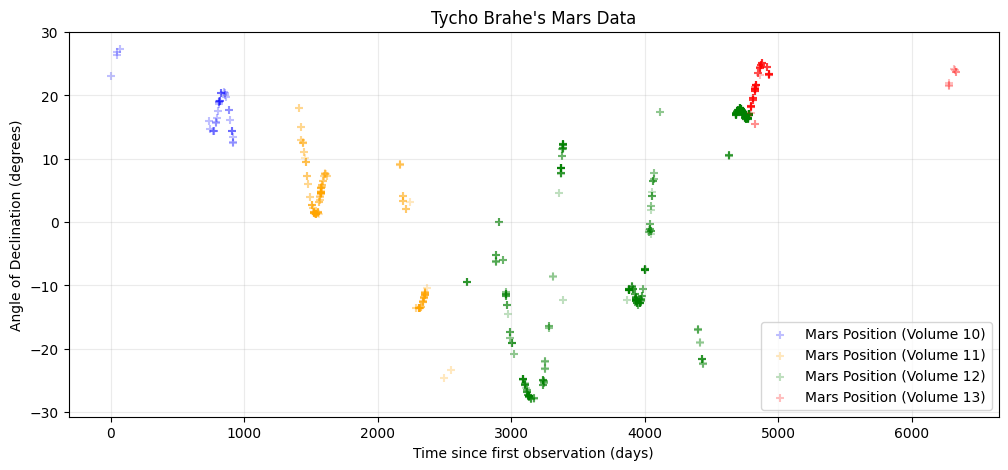
\includegraphics[scale=0.5]{images/proj00_plot_MarsDeclination.png}
\end{document}